\documentclass{article}


% if you need to pass options to natbib, use, e.g.:
%     \PassOptionsToPackage{numbers, compress}{natbib}
% before loading neurips_2022


% ready for submission
\usepackage{neurips_2022}


% to compile a preprint version, e.g., for submission to arXiv, add add the
% [preprint] option:
%     \usepackage[preprint]{neurips_2022}


% to compile a camera-ready version, add the [final] option, e.g.:
%     \usepackage[final]{neurips_2022}


% to avoid loading the natbib package, add option nonatbib:
%    \usepackage[nonatbib]{neurips_2022}


\usepackage[utf8]{inputenc} % allow utf-8 input
\usepackage[T1]{fontenc}    % use 8-bit T1 fonts
\usepackage{hyperref}       % hyperlinks
\usepackage{url}            % simple URL typesetting
\usepackage{booktabs}       % professional-quality tables
\usepackage{amsfonts}
\usepackage[pdftex]{graphicx}% blackboard math symbols
\usepackage{nicefrac}       % compact symbols for 1/2, etc.
\usepackage{microtype}      % microtypography
\usepackage{xcolor}         % colors


\title{Few-Shot Drug Discovery with Prototypical Networks}


% The \author macro works with any number of authors. There are two commands
% used to separate the names and addresses of multiple authors: \And and \AND.
%
% Using \And between authors leaves it to LaTeX to determine where to break the
% lines. Using \AND forces a line break at that point. So, if LaTeX puts 3 of 4
% authors names on the first line, and the last on the second line, try using
% \AND instead of \And before the third author name.


%\author{%
%  David S.~Hippocampus\thanks{Use footnote for providing further %information
%    about author (webpage, alternative address)---\emph{not} for %acknowledging
%    funding agencies.} \\
%  Department of Computer Science\\
%  Cranberry-Lemon University\\
%  Pittsburgh, PA 15213 \\
%  \texttt{hippo@cs.cranberry-lemon.edu} \\
  % examples of more authors
  % \And
  % Coauthor \\
  % Affiliation \\
  % Address \\
  % \texttt{email} \\
  % \AND
  % Coauthor \\
  % Affiliation \\
  % Address \\
  % \texttt{email} \\
  % \And
  % Coauthor \\
  % Affiliation \\
  % Address \\
  % \texttt{email} \\
  % \And
  % Coauthor \\
  % Affiliation \\
  % Address \\
  % \texttt{email} \\


\begin{document}
\nolinenumbers

\maketitle


\begin{abstract}
Deep neural networks (DNNs) and other probablistic techniques have demonstrated a strong ability for inferring the properties and activities of small-molecule compounds in large drug discovery datasets, but it remains in question whether or not they can reasonably be applied.  These methods typically require thousands of samples, if not millions, which is in stark contrast to most drug discovery pipelines which can only characterize compounds on the order of dozens. This makes the few-shot learning paradigm of extraordinary interest to AI-driven drug discovery. Herein, we adapt the popular meta-learning framework of prototypical networks to produce reliable predictions on chemical datasets given only a few examples. Instead of learning new classes, we show that it is possible to rapidly learn new chemical tasks despite the extremely complex task structure and vast chemical search space. Using a graph-based approach, we report a method that is compatible with molecules of any size and modality and show results on two benchmark datasets (Tox21, MUV).  Our approach offers competitive performance on the Tox21 dataset and significantly outperforms existing methods on the MUV dataset.
\end{abstract}


\section{Introduction}


All drug discovery efforts are systematically plagued by the low-data problem. This is easy to imagine, as novel, undiscovered compounds naturally have no experimental data. But this problem extends to the space of known therapeutics as well, since the expertise and expenses required to curate chemical data are astronomically larger than more accessible fields, such as natural language processing (NLP) or computer vision \cite{lusher2014data}. This makes probabilistic techniques compatible with limited data of extreme interest to chemical machine learning.


When drug discovery teams venture to find new therapeutics, the process typically results in evidence of a particular molecule carrying the capacity to modulate the desired pathway, but has one of many issues ranging from toxicity to low solubility \cite{waring2015analysis}.  The process then becomes an optimization problem, where teams experiment with chemical analogues that have the same pharmaceutical activity but minimal undesired effects.  Due to the lack of biological and chemical data on drug candidates and their analogues, this process is extremely time-consuming and expensive, and cannot currently be enriched by the recent deep learning advances that require large amounts of data.


The few-shot learning paradigm aims to work within the low data regime, by adapting a classifier to new classes not seen in training given only a few examples \cite{wang2020generalizing}.  Recent approaches \cite{DBLP:journals/corr/SnellSZ17,finn2017model,brown2020language,vinyals2016matching,ravi2016optimization} have made significant progress in showing that new classes can be efficiently and accurately learned given only a few data points, or even a single data point.  In particular, prototypical networks \cite{DBLP:journals/corr/SnellSZ17} uses the idea of a learnable embedding function in which points of a particular class cluster together. Learning this embedding function involves randomly selecting a subset of classes from the training set, then choosing a subset of examples within each class to act as the support set and a subset of the remainder to serve as query points (see Figure 1).  Learning occurs episodically, and the embedding function is adapted over episodes such that query points are accurately classified relative to the embedded support sets.

\begin{figure}
  \centering
  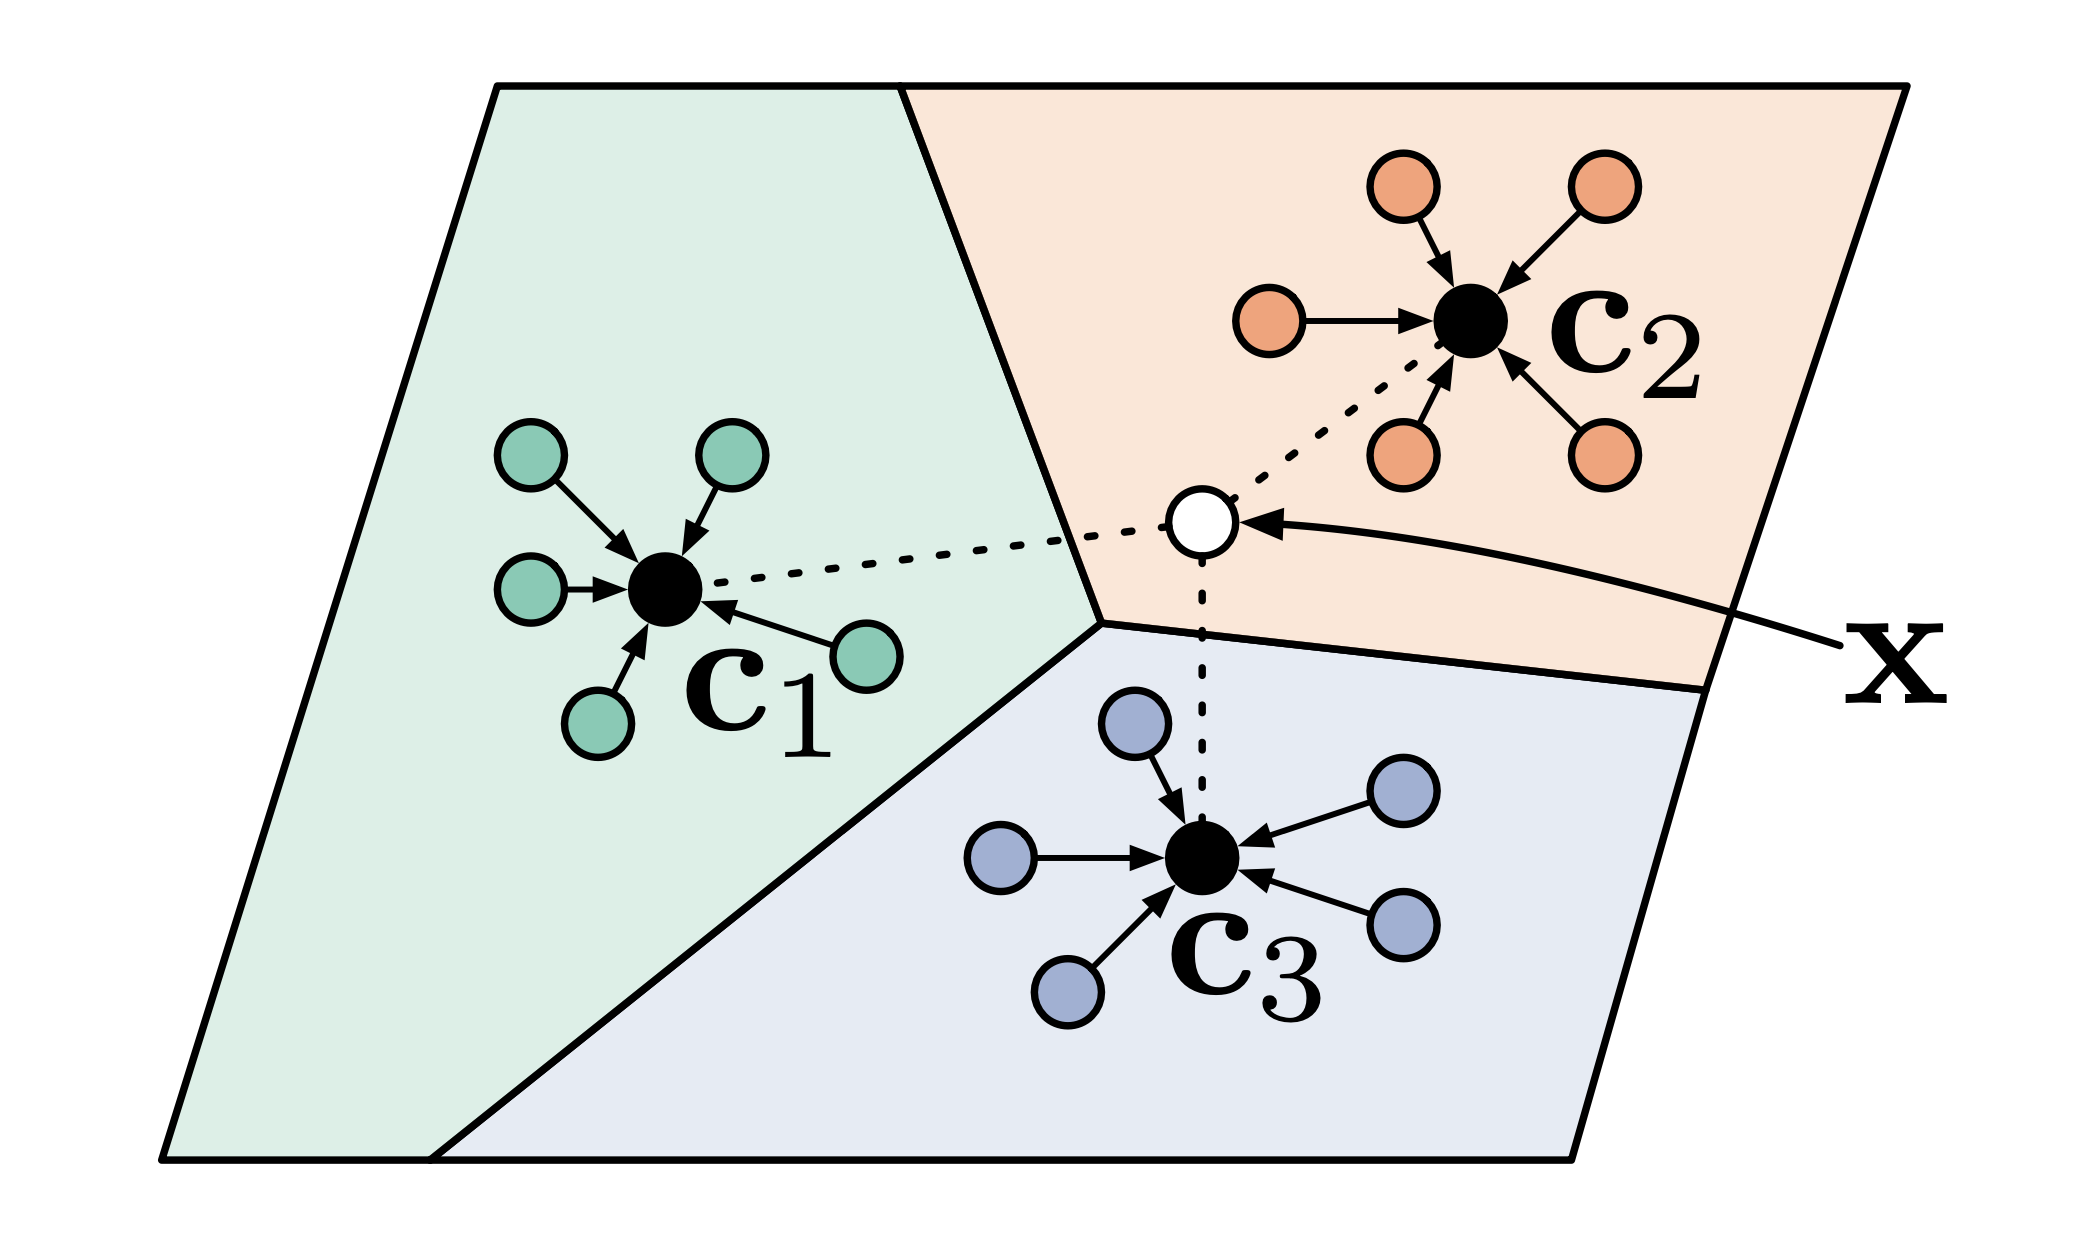
\includegraphics[width=10cm]{FINAL/Screen Shot 2022-03-22 at 11.39.35 AM.png}
  \caption{Prototypical Networks in the few-shot scenario. Prototypes $\textbf{c}_k$ are computed as the mean of embedded support examples for each class (figure from \cite{DBLP:journals/corr/SnellSZ17}).}
\end{figure}

Prototypical networks are a natural reflection of an artifact in chemical theory: similar structures typically have similar functions \cite{clayden2012organic}.  In theory, this means molecules with similar behaviors will map closely in a metric space if molecules are embedded relative to their structure. Equivalently, this means molecules could potentially be mapped from the structural space to the functional space, formalizing a structure-function relationship over compounds that is of conceptual interest, if not in the interest of few-shot classification.  


In this work, we mathematically adapt prototypical networks and the standard few-shot learning paradigm to the drug discovery problem.  We take advantage of vast literature on graph neural networks (see \cite{zhou2020graph} for review) and, in particular, use Graph Attention Networks \cite{velickovic2017graph} to design an embedding function compatible with size-variable graph representations of compounds.  Our graph-based approach allows for information between atoms and bonds to be exchanged and embedded based on their relative importance to chemical function.  Unlike the typical few-shot learning paradigm, where a classifier is adapted to recognize new classes, we show that it is possible to adapt prototypical networks to quickly learn new tasks.  In our setup, the learned embedding function is able to predict the behavior of a molecule in a new experimental system.  We report the results of our method of two datasets from the MoleculeNet \cite{wu2018moleculenet} suite of multi-task datasets, Tox21 and MUV, and achieve great results.

Outside of this work, there is only one other attempt to formally apply the few-shot learning paradigm to drug discovery, which is why a comprehensive review of previous works is not included in this report.  In Altae-Tran et. al. (2017), an iterative refinement long short-term memory network is paired with Vinyals et. al.'s (2016) matching networks to perform few-shot learning on a similar suite of datasets as those included in this study \cite{altae2017low,vinyals2016matching}.  For continuity, we follow a similar training/testing procedure that allows us to compare the results of this study with their report.  This procedure and other relevant experimental methods are described in Section 2.  Section 3 details the results of our experiments and we conclude our work in Section 4.

\section{Methods}
In this section, we mathematically formalize our few-shot learning setup, describe our application of prototypical networks, explain our choice of embedding function, and detail model training and evaluation.
\subsection{Mathematical Formalism}

Consider the situation in which one has multiple binary learning tasks.  A proportion of tasks are reserved for training, and the remaining tasks have too little data for standard machine learning models to learn an effective classifier. These remaining datasets are used for the validation sets and test sets, and the goal is to use the training tasks to create strong classifiers during validation/testing.  Our primary assumption about the tasks, and their structure, is that they are arbitrarily related.  Easier few-shot learning setups involve training tasks and test tasks that are nearly identical.  Harder few-shot learning setups feature a set of tasks that are entirely distinct from one another.


We are given $T$ tasks, each associated with a data set, $S = \{(x_i,y_i)\}^N$, where $x_i$ describes a chemical compound and $y_i \in \{0,1\}$.  We refer to the collection of available data points for a given task as a support set.  The goal is to learn a function $h$, parameterized upon support set $S$, that predicts the label of any query $x$.  Formally, $h_S(x) = \chi \to [0,1]$, where $\chi$ is the chemical space of small-molecules.  In $n$-shot learning, we have $n = |S|$ and an unbounded number of query examples.

\subsection{Prototypical Networks}

Given the setup described above, we can describe $S_k$ as the set of support examples labeled with class $k$.  If each $x_i \in \mathbb{R}^D$, we can compute an $M$-dimensional representation $\textbf{c}_k \in \mathbb{R}^M$ of each class through an embedding function $f_\Theta : \mathbb{R}^D \to \mathbb{R}^M$ with learnable parameters $\Theta$.  The representation of each class, or the prototype, is the mean vector of the embedded support points belonging to its class:


    $$\textbf{c}_k = \frac{1}{|S_k|}\sum_{\left(x_i,y_i\right) \in S_k}f_\Theta\left(x_i\right)$$


For a given query point $x$ and distance function $d : \mathbb{R}^M \times \mathbb{R}^M \to [0, \infty)$, a distribution over classes is produced based on a softmax over distances to the prototypes in the embedding space:

    $$p_\Theta\left(y = k | x\right) = \frac{\exp{-d\left(f_\Theta\left(x\right), \textbf{c}_k\right)}}{\sum_{k'}\exp{-d\left(f_\Theta\left(x\right), \textbf{c}_{k'}\right)}}$$
    
Learning proceeds through the episodic training described in Section 2.4.

\subsection{Graph Attention Networks \& Graph Encoding}
The choice of embedding function $f_\Theta : \mathbb{R}^D \to \mathbb{R}^M$ was a graph attention network (GAT), which features graph convolutions that leverage masked self-attentional layers to attend over their neighborhoods' features (see figure 2).  The input to each layer is a set of node features, $\textbf{h} = \{\vec{h}_1,\ldots,\vec{h}_N\}$, $\hat{h}_i \in \mathbb{R}^F$, where $N$ is the
number of nodes, and $F$ is the number of features in each node.  The output of each layer is a new set of node features, $\textbf{h}' = \{\vec{h}_1',\ldots,\vec{h}_N'\}$.  A shared linear transformation, with weight matrix $\textbf{W} \in \mathbb{R}^{F\times F}$ is applied to every node.  This allows for a shared attentional mechanism $a : \mathbb{R}^{F} \times \mathbb{R}^{F} \to \mathbb{R}$ to be applied and attention coefficients to be computed, yielding

$$e_{ij} = a\left(\textbf{W}\vec{h}_i,\textbf{W}\vec{h}_j\right)$$

where $i$ is any node and $j \in \mathcal{N}_i$, $\mathcal{N}_i$ being the immediate neighborhood of nodes surrounding $i$.  The attention mechanism, $a$, is a single-layer feedforward neural network,
parametrized by a weight vector $\vec{a} \in \mathbb{R}^{2F}$.  The network is followed by a LeakyReLU nonlinearity, with negative input slope $\alpha$ = 0.2.  To calculate proper node contributions, attention coefficients are normalized across all neighbors as follows:

    $$\alpha_{ij} = \frac{\exp{\left(e_{ij}\right)}}{\sum_{k\in \mathcal{N}_i}\exp{\left(e_{ik}\right)}}$$

By stacking these layers, we can turn molecules into vectorial representations.  Convolution with graphs proceeds in the same way as done with images, except the number of nodes is not predefined allowing for all compounds to be classified despite variations in size.  Our GAT model features two GAT layers with dropout (0.6) at each layer and a standard ReLU following the first layer.  After the second layer, a graph gathering layer adds together the vector of descriptors that occurs at each node as well as the vector of descriptors that occurs at each edge.  This graph gathering layer allows for an embedding of $x_i \in \mathbb{R}^D$ when $D$ is variable.  This allows us to cover the entire chemical space and reliably map $\mathbb{R}^D \to \mathbb{R}^M \ \forall \ D \in \mathbb{N}$.  The first GAT layer features eight heads, and the second GAT layer only has one head.

\begin{figure}
  \centering
  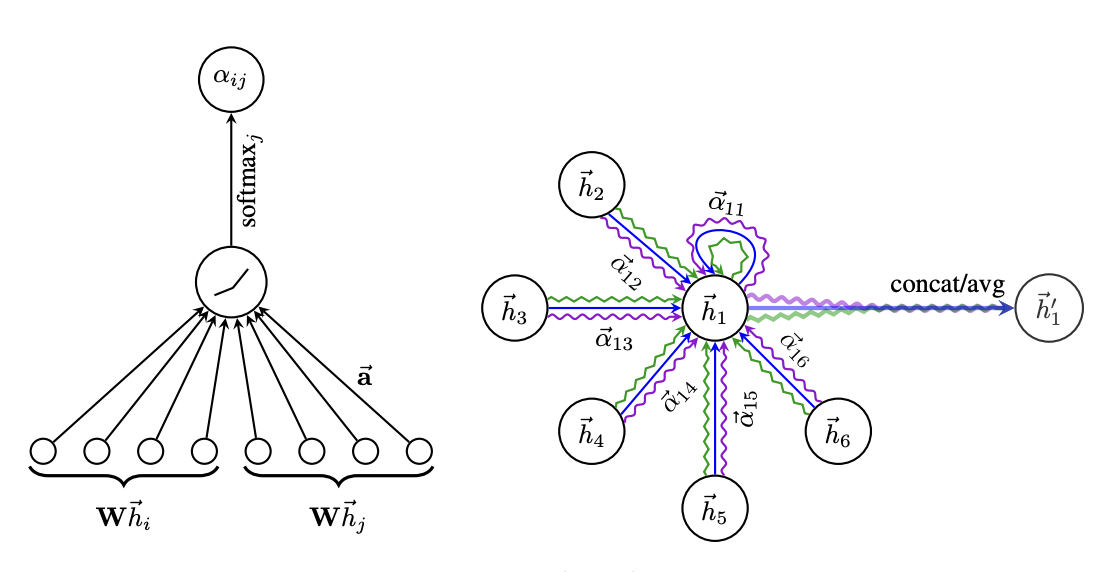
\includegraphics[width=13.5cm]{FINAL/Screen Shot 2022-04-26 at 12.10.21 AM.png}
  \caption{The left image shows attention over a set of neighbors.  The attention vector, $\vec{a}$, determines the relative weighting and a LeakyReLU activation is applied after adding together weighted nodes.  The right images shows multi-head attention (heads = 3) on a neighborhood.  Different arrow styles and colors denote independent attention computations.  $\hat{h_1'}$ is formed through this weighted aggregation of features.  Figure from \cite{velickovic2017graph}.}
\end{figure}

Each node, or atom, is encoded with information pertaining to the atom's type, degree, charge, hybridisation, whether or not it is in a ring, whether or not it is aromatic, its mass, Van der Waals radius, covalent radius, and chirality.  Each edge, or bond, is encoded with information pertaining to the bond's type, conjugacy, stereochemistry, and whether or not it helps form a ring.  At the granularity of individual atoms and bonds, this featurization encodes virtually all of the essential information that could potentially determine function at higher levels of abstraction.  By utilizing attention, the embedding function naturally selects the atom and bond configurations with the most impact towards function by effectively weighting the contribution of each neighbor when convolving.  This is critical to our goal of appropriately mapping chemical structures to a functional representation.

\subsection{Model Training and Evaluation}

As previously mentioned, the objective for our experimental setup is to learn new tasks, rather than new classes.  The goal is to transfer information between related, but distinct learning tasks, and quickly adapt.  

Let $T$ represent all tasks and $Tr$, $V$, and $Te$ represent three disjoint subsets of $T$, corresponding, respectively, to training, validation, and test sets.  Let $S$ represent a support set, and let $B$ represent a batch of queries.  We minimize the following:

    $$\mathcal{L} = -\mathbb{E}_{t\in Tr}\left[\mathbb{E}_{S\sim t, B\sim t}\left[\sum_{(x,y)\in B}\log{P_{\theta}(y|x, S)}\right]\right]$$
    
Training follows an episodic learning regime.  In each episode, a task $t\in Tr$ is randomly sampled, and then a support $S$ and a batch of queries $B$ (nonoverlapping) are sampled from the task.  One gradient descent step is taken after each episode, minimizing $\mathcal{L}$ (ADAM used as the optimizer in our setup but any SGD optimizer can be used).

At validation time and test time, a support of size $|S|$ is sampled at random for each validation and test task.  A prototype representation is calculated and evaluated with the remainder of the data points.  This procedure is done 20 times to produce the results reported below.  Validation sets are used to keep track of the best performing embedding function at the end of each epoch.  Test sets are completely held out and only used once all 2000 epochs complete. 

Models were evaluated on Tox21 and MUV.   The Tox21 collection consists of 12 nuclear receptor assays related to human toxicity.  We use the first eight assays as the training set, the ninth assay as a validation set, and the last three assays as the test set.  The MUV data set collection contains 17 assays designed to be challenging for standard virtual screening.  We use the first twelve tasks as the training set, the next two tasks as the validation set, and the last three assays as the test set.  Since these datasets are typically unbalanced due to the positive selection of compounds with desired traits, we balance the number of positive and negative examples at validation/test time to better reflect the kind of class probabilities seen in practice. 


Throughout the training procedure, we use the validation set to keep track of the best performing model configuration.  Once training is complete, we apply the best performing model and the last model on the test set.  The results reported below are all of the model achieved on the last epoch, which invariably offered the best performance.


\section{Results and Discussion}
On Tox21 and MUV datasets, we show that we are able to learn predictive embeddings given very few data points (see Tables 1,2).  These results are particular interesting, due to the amount of variance in chemical structures and associated labels.  In the Tox21 data collection, we show great performance given the limited amount of time allotted to optimize our embedding function and execute this project.  The MUV data collection is an inherently more complex learning task.  Each data point in this task is structurally distinct.  This represents the best case for standard machine learning methods, since a large portion of the chemical domain is covered.  However, this is the worst case for low-data methods because they rely heavily on similarity and relatedness to perform inference.  Yet, we were able to generally perform better with the MUV dataset than the Tox21 dataset. 


Relative to the iterative refinement long short-term memory network presented in Altae-Tran et. al. (2017), we were significantly outperformed in the simpler Tox21 but performed much better in the more complicated MUV task.  We were not able to investigate this further, but we hypothesize that the stronger inductive bias provided in Altae-Tran et. al. (2017) benefits simple tasks, whereas the weaker inductive bias of prototypical networks allows them to perform better in more complicated task structures.  Another possibility is that the vast differences in embedding functions makes performance better on some task structures and not others.  


We can see the effect of the more complicated task structure by observing the vast performance difference between large support sets and small support sets.  This gap in performance is significantly less with Tox21, an inherently simpler few-shot learning task, which offers an empirically supported heuristic: prototypical networks require a support set that is proportional to learning complexity.  This is a powerful insight that can inform chemical analyses should the techniques reported here be applied.  Instead of curating massive datasets as chemists would have to do if they wished to apply DNNs, they could use dataset sizes on the order of dozens, which is typically accessible.  While the accuracy is not perfect, this method can at least reduce the search space of drug candidates, effectively saving both time and expense.  If the experimenter wishes to achieve more accurate predictions, tremendous performance gains can be achieved with only a few more examples.  In the typical deep learning or machine learning setup, hundreds or thousands of additional examples would need to be observed in order to see any performance gains.

The results of both datasets demonstrate the central objective of few-shot learning: given a plentiful amount of out-of-domain data, we can learn a classifier that can quickly adapt to the relavant task using the limited amount of in-domain data.

\begin{table}
  \caption{Accuracy of Models on Median Held-out Task (Tox21). Numbers reported are means and standard deviations. Randomness is over the choice of support set; experiment is repeated with 20 support sets.}
  \label{sample-table}
  \centering
  \begin{tabular}{lll}
    \toprule
    Pos/Neg & \textbf{ProtoGAT (this study)} & IterRefLSTM (Altae-Tran et. al., 2017) \\
    \midrule
    -20/+20 & 0.618 $\pm$ 0.003 & -     \\
    -10/+10 & 0.607 $\pm$ 0.005 & 0.823 $\pm$ 0.002      \\
    -5/+5   & 0.581 $\pm$ 0.008 & -  \\
    -1/+1   & 0.547 $\pm$ 0.004 & 0.827 $\pm$ 0.001  \\
    \bottomrule
  \end{tabular}
\end{table}

\begin{table}
  \caption{Accuracy of Models on Median Held-out Task (MUV). Numbers reported are means and standard deviations. Randomness is over the choice of support set; experiment is repeated with 20 support sets.}
  \label{sample-table}
  \centering
  \begin{tabular}{lll}
    \toprule
    Pos/Neg & \textbf{ProtoGAT (this study)} & IterRefLSTM (Altae-Tran et. al., 2017) \\
    \midrule
    -20/+20 & 0.722 $\pm$ 0.049 & -     \\
    -10/+10 & 0.643 $\pm$ 0.031 & 0.499 $\pm$ 0.053      \\
    -5/+5   & 0.617 $\pm$ 0.023 & -  \\
    -1/+1   & 0.539 $\pm$ 0.019 & 0.479 $\pm$ 0.037  \\
    \bottomrule
  \end{tabular}
\end{table}

\section{Conclusion}


We have proposed an adaptation to prototypical networks that allows molecules to be represented and featurized as graphs and for few-shot learning to be conducted via a representation space.  We demonstrated that these networks perform well on the Tox21 dataset, and significantly outperform existing methods on the MUV dataset.  Moreover, we show that the few-shot learning paradigm cannot only be used to quickly learn new classes, but new tasks as well.


In the spirit of not only concluding this report, but this class, we would like to use this final section to 1) explicitly mention the probabilistic techniques taught in class that appeared in this project, 2) discuss the future work that should be done if this project continued towards a meaningful publication.  A tremendous amount of work and effort was put into this project, and hopefully I will have time this summer to explore the directions mentioned below.


Graph neural networks are obviously a probabilistic technique, and one mentioned in this class (briefly), and were used heavily in this project.  However, the main idea, being prototypical networks, is deeply rooted as a probabilistic technique.  When using a particular class of distance functions known as regular Bregman divergences, prototypical networks are equivalent to performing mixture density estimation on the support set with an exponential family density.  When using Euclidean distance as the distance function, as done in this project, prototypical networks can be casted as a linear model.  For brevity, we refer the reader to \cite{DBLP:journals/corr/SnellSZ17} for a more detailed treatment of these ideas.


There are several interesting and meaningful avenues to be taken that can turn this report into a publishable work.  First, it would be very interesting to visualize prototypes and embeddings using probablaitic PCA \cite{tipping1999probabilistic} and/or t-sne \cite{van2008visualizing}.  Unfortunately, we did not have time to complete this somewhat complicated procedure for chemical embeddings.  Second, it would greatly benefit the method to optimize the embedding network.  The choice of a graph attention network was somewhat arbitrary, and the focus of this report was on the adaptation of prototypical networks for chemical data.  Our choice of embedding function has room for improvement, and that should be explored.  Third, a more comprehensive comparison of few-shot learning approaches should be conducted.  This included comparing different embedding functions with the prototypical setup and possibly implementing a few-shot random forests model.  This would give the reader a more complete picture, but was clearly not possible for this report given the time restraints.  Lastly, exploring more datasets is a must.  

\section*{Acknowledgements \& Final Remarks}
We would like to thank Dr. Adji Bousso Dieng for the conversations and lecture material that provided a lot of intuition when completing this project.  Prior to adding tables and figures, this report was just under 5 pages.  We deliberately omitted several sections in this report to avoid violating the page restriction: a comprehensive treatment of graph attention networks, review of AI-driven drug discovery.  We attempted to focus on the probabilistic techniques relevant to the course.  

\bibliographystyle{unsrt}
\bibliography{refs}

\end{document}